\section{\astarix: Finding Optimal Alignments Using \A} \label{sec:astarix-algo}
In this section, we first introduce the general \A algorithm for finding
shortest paths, and the notion of an optimistic heuristic, a sufficient
condition for instantiations of \A to be correct (i.e., to indeed find shortest
paths). Then we instantiate \A with our domain-specific heuristic that accounts
for upcoming subsequences to be aligned, and prove that this heuristic is
optimistic.

\begin{algorithm}[t]
	\caption{\astarix including heuristic function.}\label{alg:astarix}
	\begin{algorithmic}[1]
		\State $\RG$: Reference graph \label{lin:reference}
		\Comment Global variables
		\State $d$: Upcoming sequence length \label{lin:d}
		\Statex
		\Function{AStarix}{$q\colon \text{Query}$} \label{lin:astarix}
			\State $\AG \gets \Call{DefineAlignmentGraph}{\RG, q}$
			\Comment Following \cref{sec:task}
			\State $S \gets \{\langle v,i \rangle \in \AGV \mid i=0 \}$ \label{lin:starts}
			\Comment Sources: no letter matched
			\State $T \gets \{\langle v,i \rangle \in \AGV \mid i=|q| \}$
			\Comment Targets: all letters matched
			\State \Return $\Call{\A}{\AG, S, T, \textsc{Heuristic}}$
			\Comment \A provided in \cref{app:astar} \label{lin:ret}
		\EndFunction
		\Statex
		\Function{Heuristic}{$\langle u, i \rangle\colon \text{State}$} \label{lin:heuristic-start}
		\Comment Heuristic: Cost of upcoming sequence
			\State $d' \gets \min(d, |q|-i)$
			\Comment Actual length of upcoming sequence
			\State $s \gets q[i:i+d']$ \label{lin:s}
			\Comment Upcoming sequence (next $d$ letters after current)
			\State \Return $\Call{$h$}{u, s}$
			\label{lin:align-upcoming}
			\Comment Cost of aligning $s$ to $\EG$ starting from $u$
		\EndFunction \label{lin:heuristic-end}
		\Statex
		\Function{$h$}{$u, s$}
		\Comment Cost of aligning $s$ starting from $u$
			\State \Return $\Call{RecursiveAlign}{u, s, 0.0, \infty}$
			\Comment Simple branch-and-bound \label{lin:recursive-align}
		\EndFunction
	\end{algorithmic}
\end{algorithm}
\subsection{Background: General \A algorithm} \label{subsec:general-astar}
Given a weighted graph $G=(V,E)$ with $E \subseteq V \times V \times
\mathbb{R}_{\geq 0}$, the \A algorithm (abbreviated as \A) searches for the
shortest path from sources $S \subseteq V$ to targets $T \subseteq V$. It is an
extension of Dijkstra's algorithm that additionally leverages a \emph{heuristic
function} $h \colon V \to \mathbb{R}_{\geq 0}$ to decide which paths to explore
first.
%
If $h(u) \equiv 0$, \A is equivalent to Dijkstra's algorithm.
%
We provide an implementation of \A and Dijkstra in \cref{app:astar}, but do not
assume knowledge of either algorithm in the following.
%
At a high level, \A maintains the set of all \emph{explored} states, initialized
with the set of sources $S$. Then, \A iteratively \emph{expands} the explored
state with lowest estimated cost by exploring all its neighbors, until it finds
a target. Here, the cost for node $u$ is estimated by the distance from source, called $g(u)$, plus the estimate from the heuristic $h(u)$.


\para{Heuristic Function}
The heuristic function $h(u)$ estimates the
cost $h^*(u)$ of a shortest path in $G$ from $u$ to a target $t \in T$. Intuitively, a
good heuristic correlates well with the distance from $u$ to $t$.

To ensure that \A indeed finds the shortest path, $h$ should be
\emph{optimistic}:

\begin{definition}[Optimistic heuristic] A heuristic $h$ is \textit{optimistic}
    if it provides a lower bound on the distance to the closest target: $\forall u. h(u) \leq h^*(u)$.
\end{definition}

While any optimistic $h$ ensures that \A finds optimal
alignments~\cite{dechter_generalized_1985}, the specific choice of $h$
is critical for performance. In particular, decreasing the error $\delta(u) =
h^*(u)-h(u)$ can only improve the performance of
\A~\cite{dechter_generalized_1985}. Thus, a key contribution of ours is
a domain-specific heuristic $h$.


\subsection{\astarix: Instantiating \A} \label{TRIEsubsec:astarix-heuristic}
\cref{TRIEalg:astarix} shows an unoptimized version of \astarix and its heuristic
function.
%
\astarix expects a reference graph (\cref{TRIElin:reference}) and a query
(\cref{TRIElin:astarix}) as input, and returns an optimal alignment (\cref{TRIElin:ret})
by searching for a shortest path from $S$ to $T$ in the alignment graph $\AG$.
It is parameterized by hyper-parameters ($d$ in \cref{TRIElin:d}, more in
\cref{TRIEsec:optimizations}) and edit costs (implicitly provided).

The function \textsc{Heuristic}
(\crefrange{TRIElin:heuristic-start}{TRIElin:heuristic-end}) computes a lower bound on
the remaining cost of a best alignment: the minimum cost $h(u,s)$ of aligning
the \emph{upcoming sequence} $s$ (where $\lvert s \rvert \leq d$) starting from
node $u$. Importantly, $s$ is limited to the next $d' \leq d$ letters of $q$,
starting from query position $i$. Thus, computing $h(u,s)$ is substantially
cheaper than aligning all remaining letters of $q$.

To compute $h(u,s)$ we leverage a simple branch-and-bound algorithm, provided in
\cref{TRIEapp:recursive-align}. In the following, for convenience, we refer to the
heuristic as $h$ (which is parameterized by $(u,s)$) instead of
\textsc{Heuristic} (which is parameterized by $\langle u, i \rangle$). Further,
we say that $h$ is optimistic if $h(u,s)$ is a lower bound on the cost for
aligning all remaining letters (\ie, $q[i:|q|]$) starting from node $u$ (note
that $s$ is a prefix of $q[i:|q|]$).

\begin{samepage}
\begin{thm} \label{TRIEthm:optimistic}
	$h$ is optimistic.
\end{thm}
\begin{proof}
$h$ only considers the next $d'$ letters of $q$ instead of all
remaining letters. Since all costs are non-negative, the theorem follows.
\end{proof}
\end{samepage}

\begin{figure}[t]
	\centering
	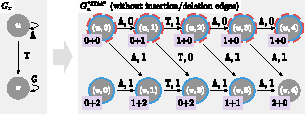
\includegraphics[width=0.9\columnwidth]{figs/heuristic}
	\caption{The benefit of using our heuristic over \dijkstra. Alignment graph
	$\AG[``\texttt{ATAA}"]$ (right) is based on reference graph $\RG$ (left),
	but omits insertion and deletion edges for simplicity. The pink boxes $g+h$
	indicate the distance from the sources $S=\{\langle u,0 \rangle, \langle v,0
	\rangle \}$ (in $g$) and the cost of aligning the next $d=2$ letters (in
	$h$). \dijkstra (resp. \A) expands states circled in
	\textcolor{my-full-blue}{blue} (resp.
	\textcolor{my-full-red}{dashed red}).}
	\label{TRIEfig:heuristic-benefit}
\end{figure}

\para{Benefit of \A Heuristic over \dijkstra} \label{TRIEpara:heuristic-benefits}
\cref{TRIEfig:heuristic-benefit} shows the benefit of using our heuristic function
compared to \dijkstra. Here, \dijkstra expands states based on their distance
$g$ from the origin nodes $\st{u}{0}$ and $\st{v}{0}$. Hence, depending on
tie-breaking, \dijkstra may expand all states with $h \leq 1$, as shown in
\cref{TRIEfig:heuristic-benefit}. By contrast, \A chooses the next state to expand
by the sum of the distance from the origin $g$ and the heuristic $h$, expanding
only states with $g+h \leq 1$.

\para{Memoization} \label{TRIEpara:memoization}
Recall that the return value of $h$ in \cref{TRIElin:heuristic-start} only depends
on $u$ and the upcoming sequence $s$ (which in turn depends on $i$ and $d$).
Thus, $h(u,s)$ can be reused for different positions across different queries in
$\Oh(1)$ time, if it was computed for a previous query.
\section{Optimizations} \label{TRIEsec:optimizations}

We now discuss several optimizations we developed to speed up \astarix while
preserving its optimality. These optimizations reduce preprocessing and
alignment runtime as well as memory footprint (in particular for memoization).
Our aligner \astarix handles both \A and \dijkstra algorithm (formally with $h
\equiv 0$).

\subsection{Greedy match optimization} \label{TRIEsubsec:greedy}
We also employ an optimization originally developed for computing the edit
distance between two strings~\cite{sellers_algorithm_1974,allison_lazy_1992}, but
which has also been used in the context of string to graph
alignment~\cite{dox2018efficient}. We omit the correctness proof of this
optimization, which is already covered
in~\cite{sellers_algorithm_1974}, and only explain the intuition behind it.

Suppose there is only one outgoing edge $e = (u, v, \ell) \in \RGE$ from a node
$u \in \RGV$. Suppose also that while aligning a query $q$, we explore state
$\st{u}{i}$ for which the next query letter $q[i]$ matches the label $\ell$. In
this case, we do not need to consider the edit outgoing edges, because
any edit at this point can be postponed without additional cost, as $\cmatch
\leq \min(\csubst, \cins, \cdel)$. Thus, we can greedily explore state
$\st{v}{i+1}$, aligning $q[i+1]$ to $e$ by using the edge $(\st{u}{i},
\st{v}{i+1}, \ell, \cmatch)$ before continuing with the \A search.
We note that this optimization is only applicable when aligning in non-branching
regions of the reference graph. In particular, it is not applicable for most
trie nodes (\cref{TRIEsubsec:trie}).

\subsection{Capping the cost and depth} \label{TRIEsubsec:speedup-heuristic}
In the following, we show how to reduce the runtime of evaluating the heuristic
$h(u,s)$, by introducing two separate optimizations that compose naturally.

\paragraph{Capping cost} We cap $h(u,s)$ at $\costcap$, replacing it by
$h_{\costcap}(u,s):=\min(h(u,s),\costcap)$. To achieve this, we allow
\textsc{RecursiveAlign} to ignore paths costing more than $\costcap$.
%
For large enough $\costcap$, this speeds up computation without significantly
decreasing the benefit of the heuristic, since nodes associated with a high
heuristic value are typically not explored anyways. We investigate the effect of
$\costcap$ in \cref{TRIEsubsec:parameter_estimation}.

\begin{samepage}
	\begin{thm} \label{TRIEthm:hcostcap_admissible}
		$h_{\costcap}$ is admissible.
	\end{thm}
	\begin{proof}
		Follows from $h_\costcap(u,s) \leq h(u,s)$ and $h(u,s)$ being admissible
		(\cref{TRIEthm:admissible}).
	\end{proof}
	\end{samepage}

\paragraph{Capping depth}
We reduce the number of nodes that need to be considered by $h(u,s)$. To this
end, we define a modified heuristic $h_d(u,s)$ that only considers nodes $R_u
\subseteq \AGV$ at distance at most $d$ from $u$ (in \cref{TRIEalg:astarix}):
$
R_u := \{ v \in \RGV \mid \exists \; \text{path } \pi \in \RG \text{ from } u \text{ to } v \text{ with } \lvert \pi \rvert \leq d \}
$.

If an alignment of $s$ reaches the boundary of $R_u$, defined as $$B(R_u) := \{v
\in R_u \mid \exists (v,v',\ell) \in \AGE \text{ with } v' \notin R_u \},$$ it is
allowed to only spell a prefix of $s$, and the remaining unaligned letters of
$s$ are considered aligned with zero cost:
\begin{gather*}
h_d(u,s) := \min_{\pi \in \Pi} \cost{\pi}, \text{ where } \\
\Pi := \left\{ \pi \in \RG \;\middle|\;
%\begin{array}{c}
\mli{start}(\pi)=u, 
\sigma(\pi)=s \lor \big(\mli{end}(\pi)\in B(R_u) \land \exists i. \sigma(\pi)=s[1..i] \big)
%\end{array}
\right\}
\end{gather*}

\begin{samepage}
\begin{thm} \label{TRIEthm:hbar_admissible}
	$h_d$ is admissible.
\end{thm}
\begin{proof}
	It suffices to show $h_d(u,s) \leq h(u, s)$ since $h(u, s)$ is admissible.
	In the case where all of $s$ is aligned, $h_d(u,s) = h(u, s)$. Otherwise,
	the unaligned letters of $s$ are not penalized, so $h_d(u,s) \leq h(u, s)$.
\end{proof}
\end{samepage}


\subsection{Equivalence classes} \label{TRIEsubsec:partition}

We have shown in \cref{TRIEpara:memoization} how to reuse an already computed
$h(u,s)$ for repeating $s$ across different queries and query positions. In the
following, we additionally aim to reuse $h(u,s)$ across different nodes $u$, so
that $h(u,s)$ does not need to be computed for all nodes $u$. Intuitively, we
want to assign two nodes $u$ and $v$ to the same equivalence class when the
\emph{graph region} considered by $h(u,s)$ is equivalent to the graph region
considered by $h(v,s)$, up to renaming of nodes.

Thus, $h(u,s)=h(v,s)$ if $u$ and $v$ are from the same equivalence class.
Therefore, we can (arbitrarily) choose a representative node $r \in \RGV$ for
every equivalence class, and evaluate $h(r,s)$ instead of $h(u,s)$, where $r$ is
the representative of the equivalence class of $u$. To look up representative
nodes in $\Oh(1)$, we define a helper array $\mli{repr}$ with $\mli{repr[u]} =
r$.

\paragraph{Identifying equivalence classes}
To identify the nodes belonging to the same equivalence class, we assume the
optimization from \cref{TRIEsubsec:speedup-heuristic}, \ie, that our heuristic only
considers nodes up to a distance $d$ from~$u$.
%
Moreover, for performance reasons, our implementation detects only the
equivalence classes of nodes $u$ with a single outgoing path of length at least
$d$.
%
In this case, $u$ and $u'$ are in the same equivalence class if their outgoing
paths spell the same sequence.
%
In contrast, we leave nodes with forking paths in separate equivalence classes.

Note that for smaller $d$, the number of equivalence classes gets smaller, the
reuse of the heuristic gets higher, and the memoization table has a lower memory
footprint. At the same time, however, the heuristic $h_d(u,s)$ is less
informative.

\subsection{Data structures}
Our \astarix implementation uses an adjacency list graph data structure to
represent the reference and the trie in a unified way, representing each letter
by a separate edge object. To represent the reverse complementary walks in
$\RG$, the nodes are doubled, connected in the opposite direction, and
labeled with complementary nucleotides ($\texttt{A} \leftrightarrow \texttt{T}$,
$\texttt{C} \leftrightarrow \texttt{G}$). We do not limit the number of memoized
heuristic function values (\cref{TRIEpara:memoization}), but note we could do so
by resetting the memoization table periodically.